\documentclass[10pt]{beamer}

% ------------------------------------------------------------------------
% Carga de tu preámbulo personalizado (preamble.tex).
% Asegúrate de tenerlo junto a este archivo para que \input funcione.
% ------------------------------------------------------------------------
\usetheme[progressbar=frametitle]{metropolis}
\usepackage{appendixnumberbeamer}
\usepackage{fancyvrb}
\usepackage{booktabs}
\usepackage[scale=2]{ccicons}
\usepackage{pgfplots}
\usepgfplotslibrary{dateplot}
\usepackage{type1cm}
\usepackage{lettrine}
\usepackage{ragged2e}
\usepackage{xspace}
\newcommand{\themename}{\textbf{\textsc{metropolis}}\xspace}
\usepackage{graphicx} % Allows including images
\usepackage{booktabs} % Allows the use of \toprule, \midrule and \bottomrule in tables
\usepackage[utf8]{inputenc} %solucion del problema de los acentos.
\usepackage{xcolor}
\definecolor{LightGray}{gray}{0.9}

\usepackage{minted}
\usemintedstyle{tango}
\newcommand{\mypyfile}[1]{\inputminted[linenos=true, fontsize=\footnotesize, frame=lines, framesep=5\fboxrule,framerule=1pt]{python}{#1}}

\setminted[python]{breaklines,frame=lines,framesep=2mm,baselinestretch=1.2,bgcolor=LightGray,linenos, fontsize=\footnotesize} % obeytabs=true, tabsize=2, showtabs=true}

%%%%%%%%%%%%%%%%%%%%%%%%%%%%%%%%%%%%%%%%%%%%%%%%%%%%%%%%%%%%%%%%%%%%%%%%%%%%%%%%%%%%%%
\setbeamercolor{progress bar}{fg=blue!50!black,bg=white!50!black}
\setbeamercolor{title separator}{fg=red!50!black,bg=white!50!black}
\setbeamercolor{frametitle}{fg=white!80!black,bg=red!50!black}
\title[PCFI161]{Programaci\'on para F\'isica y Astronom\'ia}
\subtitle{Departamento de Física.}

\newcommand{\myfront}{
\author[PCFI161]{Corodinadora: C Loyola \\ Profesoras/es C Loyola / C Femenías / Y Navarrete / C Ruiz}
\institute[UNAB]{Universidad Andrés Bello}
\date{Primer Semestre 2025}
}

\titlegraphic{%
  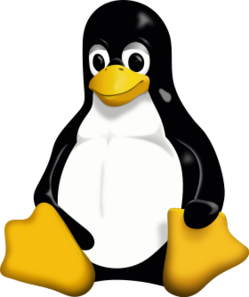
\includegraphics[width=.08\textwidth]{logo-tux.png}\hfill
  
\includegraphics[width=.3\textwidth]{logo-unab.png}\hfill
  
\includegraphics[width=.08\textwidth]{logo-python.png}
}

\makeatletter
\setbeamertemplate{title page}{
  \begin{minipage}[b][\paperheight]{\textwidth}
    \vfill%
    \ifx\inserttitle\@empty\else\usebeamertemplate*{title}\fi
    \ifx\insertsubtitle\@empty\else\usebeamertemplate*{subtitle}\fi
    \usebeamertemplate*{title separator}
    \ifx\beamer@shortauthor\@empty\else\usebeamertemplate*{author}\fi
    \ifx\insertdate\@empty\else\usebeamertemplate*{date}\fi
    \ifx\insertinstitute\@empty\else\usebeamertemplate*{institute}\fi
    \vfill
    \ifx\inserttitlegraphic\@empty\else\inserttitlegraphic\fi
    \vspace*{1cm}
  \end{minipage}
}
\makeatother


\makeatletter
\setlength{\metropolis@titleseparator@linewidth}{2pt}
\setlength{\metropolis@progressonsectionpage@linewidth}{2pt}
\setlength{\metropolis@progressinheadfoot@linewidth}{2pt}
\makeatother


\begin{document}

% ------------------------------------------------------------------------
% Portada de la Presentación
% ------------------------------------------------------------------------
\myfront{}

% ------------------------------------------------------------------------
% Slide 1: Título de la Sesión
% ------------------------------------------------------------------------
\begin{frame}
  \titlepage
  % Ejemplo:
  % \title{Semana 9 - Sesión 1 (Sesión 17): Profundizando en Programación Orientada a Objetos}
\end{frame}

% ------------------------------------------------------------------------
% Slide 2: Índice / Tabla de Contenidos
% ------------------------------------------------------------------------
\begin{frame}
  \frametitle{Resumen - Semana 9, Sesión 1 (Sesión 17)}
  \tableofcontents
\end{frame}

% ------------------------------------------------------------------------
% Configuración de bloques
% ------------------------------------------------------------------------
\metroset{block=fill}

% ----------------------------------------------------------------------------------------
% SECCIÓN 1: Introducción y Conexión con Sesiones Previas
% ----------------------------------------------------------------------------------------
\section{Introducción y Repaso}

% ------------------------------------------------------------------------
% Slide 3: Repaso de las Semanas Anteriores
% ------------------------------------------------------------------------
\begin{frame}{Repaso de las Semanas 7 y 8}
  \begin{itemize}
    \item \textbf{Semana 7}:
      \begin{itemize}
        \item Gráficos avanzados con Matplotlib (subplots, histogramas, 3D).
        \item Pequeña introducción a \texttt{pandas} para cargar/analizar datos.
      \end{itemize}
    \item \textbf{Semana 8}:
      \begin{itemize}
        \item Iniciamos POO (clases, métodos, atributos) y su uso con NumPy/pandas.
        \item Evaluaciones prácticas en clase (problemas integradores subidos a CANVAS).
      \end{itemize}
    \item \textbf{Objetivo de hoy}: Profundizar en \textbf{POO} con temas como \textit{herencia} y métodos especiales, y repasar ejemplos de uso en la Física/Astronomía.
  \end{itemize}
\end{frame}

% ------------------------------------------------------------------------
% Slide 4: Objetivos de la Sesión 17
% ------------------------------------------------------------------------
\begin{frame}{Objetivos de la Sesión 17}
  \begin{itemize}
    \item \textbf{Revisar} la retroalimentación general de las últimas evaluaciones.
    \item \textbf{Profundizar} en POO:
      \begin{itemize}
        \item Herencia y clases derivadas.
        \item Métodos especiales: \_\_str\_\_, \_\_repr\_\_, etc.
      \end{itemize}
    \item \textbf{Aplicar} estos conceptos en un ejemplo físico/astronómico (sistema de partículas derivadas, o similar).
    \item \textbf{Ejercitar} con un problema final que combine herencia con algún cálculo numérico.
  \end{itemize}
\end{frame}

% ----------------------------------------------------------------------------------------
% SECCIÓN 2: Retroalimentación de Evaluaciones Recientes
% ----------------------------------------------------------------------------------------
\section{Retroalimentación}

% ------------------------------------------------------------------------
% Slide 5: Retroalimentación General
% ------------------------------------------------------------------------
\begin{frame}{Retroalimentación de las Evaluaciones}
  \begin{itemize}
    \item \textbf{Problemas integradores} (semanas 7 y 8):
      \begin{itemize}
        \item Mayoría cumplió con generar los gráficos requeridos (histogramas, scatter, etc.).
        \item Algunos omitieron detalles de etiquetado o usaron pocas leyendas.
        \item Tiempo (25-30 min) fue suficiente en la mayoría de los casos, aunque un par de grupos tuvo problemas de último minuto.
      \end{itemize}
    \item \textbf{Áreas a reforzar}:
      \begin{itemize}
        \item Limpieza y claridad del código (comentarios / secciones).
        \item Mejor aprovechamiento de \texttt{pandas} para leer y filtrar datos.
        \item Exploración más profunda de Matplotlib (colormaps, layouts).
      \end{itemize}
  \end{itemize}
\end{frame}

% ------------------------------------------------------------------------
% Slide 6: Consejos para Mejorar
% ------------------------------------------------------------------------
\begin{frame}{Consejos para Mejorar}
  \begin{itemize}
    \item \textbf{Planificar} la estructura antes de codificar (pseudocódigo o diagrama rápido).
    \item Usar \textbf{subplots} con \texttt{fig, axs = plt.subplots()} y clarificar cada panel.
    \item Mantener un \textbf{estilo consistente}: nombres de variables, sangría, etc.
    \item Ver ejemplos oficiales de \textbf{Matplotlib} (Gallery) y \textbf{pandas} (10 minutes to pandas).
    \item Practicar \textbf{manejo de excepciones} al leer datos (opcional).
  \end{itemize}
\end{frame}

% ----------------------------------------------------------------------------------------
% SECCIÓN 3: Profundizando en Programación Orientada a Objetos
% ----------------------------------------------------------------------------------------
\section{POO Avanzado}

% ------------------------------------------------------------------------
% Slide 7: Herencia en Python
% ------------------------------------------------------------------------
\begin{frame}[fragile]{Herencia (Inheritance)}
\begin{minted}[
  frame=lines,
  framesep=2mm,
  fontsize=\footnotesize,
  bgcolor=LightGray
]{python}
class BaseClass:
    def __init__(self, name):
        self.name = name
    
    def show_info(self):
        print(f"Base Name: {self.name}")

class DerivedClass(BaseClass):
    def __init__(self, name, extra):
        super().__init__(name)  # llama al constructor de la base
        self.extra = extra
    
    def show_info(self):
        super().show_info()
        print(f"Extra info: {self.extra}")

# Uso
obj = DerivedClass("MiObjeto", 123)
obj.show_info()
\end{minted}
\begin{itemize}
  \item \textbf{DerivedClass} hereda atributos/métodos de \textbf{BaseClass}.
  \item \texttt{super()} para invocar constructor y métodos de la clase base.
\end{itemize}
\end{frame}

% ------------------------------------------------------------------------
% Slide 8: Ejemplo Físico: Particle y ChargedParticle
% ------------------------------------------------------------------------
\begin{frame}[fragile]{Ejemplo: Herencia con Partículas}
\begin{minted}[
  frame=lines,
  framesep=2mm,
  fontsize=\footnotesize,
  bgcolor=LightGray
]{python}
import math

class Particle:
    def __init__(self, mass, x, y):
        self.mass = mass
        self.x = x
        self.y = y

    def kinetic_energy(self, vx, vy):
        return 0.5 * self.mass * (vx**2 + vy**2)

class ChargedParticle(Particle):
    def __init__(self, mass, x, y, charge):
        super().__init__(mass, x, y)
        self.charge = charge

    def potential_energy(self, E_field):
        # Ejemplo: E_field as a tuple (Ex, Ey)
        Ex, Ey = E_field
        # Energia potencial ~ q * (E dot position), simplificado
        return self.charge * (Ex*self.x + Ey*self.y)
\end{minted}
\end{frame}

% ------------------------------------------------------------------------
% Slide 9: Métodos Especiales (\_\_str\_\_, \_\_repr\_\_, etc.)
% ------------------------------------------------------------------------
\begin{frame}[fragile]{Métodos Especiales en Python (Dunder Methods)}
\begin{minted}[
  frame=lines,
  framesep=2mm,
  fontsize=\footnotesize,
  bgcolor=LightGray
]{python}
class Particle:
    def __init__(self, mass, x, y):
        self.mass = mass
        self.x = x
        self.y = y

    def __str__(self):
        # String informal
        return f"Particle(m={self.mass}, x={self.x}, y={self.y})"

    def __repr__(self):
        # Representación más técnica (por defecto en las listas, etc.)
        return f"Particle(mass={self.mass}, x={self.x}, y={self.y})"
\end{minted}
\begin{itemize}
  \item \textbf{\_\_str\_\_} se usa en \texttt{print(obj)}, \_\_repr\_\_ en representaciones formales (consola, debugging).
  \item Otros métodos: \_\_eq\_\_, \_\_lt\_\_, \_\_add\_\_, etc.
\end{itemize}
\end{frame}

% ----------------------------------------------------------------------------------------
% SECCIÓN 4: Ejemplo Avanzado y Ejercicios
% ----------------------------------------------------------------------------------------
\section{Ejemplo y Ejercicios}

% ------------------------------------------------------------------------
% Slide 10: Ejemplo Combinado (POO + NumPy)
% ------------------------------------------------------------------------
\begin{frame}[fragile]{Sistema de Partículas con Herencia}
\begin{minted}[
  frame=lines,
  framesep=2mm,
  fontsize=\footnotesize,
  bgcolor=LightGray
]{python}
import numpy as np

class Particle:
    def __init__(self, mass, pos):
        self.mass = mass
        self.pos = np.array(pos, dtype=float)  # [x, y]

    def distance(self, other):
        return np.linalg.norm(self.pos - other.pos)

class ChargedParticle(Particle):
    def __init__(self, mass, pos, charge):
        super().__init__(mass, pos)
        self.charge = charge

    def electrostatic_potential(self, other, k=1.0):
        # k=1.0: factor de Coulomb simplificado
        r = self.distance(other)
        if r == 0:
            return np.inf
        return k * (self.charge * other.charge) / r
\end{minted}
\end{frame}

% ------------------------------------------------------------------------
% Slide 11: Uso e Interpretación
% ------------------------------------------------------------------------
\begin{frame}[fragile]{Uso e Interpretación}
\begin{minted}[
  frame=lines,
  framesep=2mm,
  fontsize=\footnotesize,
  bgcolor=LightGray
]{python}
p1 = ChargedParticle(mass=1.0, pos=[0,0], charge=2.0)
p2 = ChargedParticle(mass=2.0, pos=[3,4], charge=-1.0)

dist = p1.distance(p2)  # 5.0
print("Distancia:", dist)

pot = p1.electrostatic_potential(p2, k=9e9)  # coulomb k ~ 9e9 (SI units)
print("Potencial electrostático:", pot)
\end{minted}
\begin{itemize}
  \item Ejemplo sencillo, pero ilustra \textbf{herencia} (\texttt{ChargedParticle} derivada de \texttt{Particle}).
  \item Podríamos extender con listas de partículas, etc.
\end{itemize}
\end{frame}

% ------------------------------------------------------------------------
% Slide 12: Ejercicio 1 - Herencia Simple
% ------------------------------------------------------------------------
\begin{frame}{Ejercicio 1: Clase Base y Clase Derivada}
  \begin{block}{Enunciado}
    \begin{itemize}
      \item Crear una clase base \textbf{Body} con atributos (\texttt{name, mass, pos}).
      \item Crear una clase derivada \textbf{Star} (por ejemplo) con atributo adicional \texttt{luminosity}.
      \item Métodos:
        \begin{itemize}
          \item \texttt{distance(other)} en \textbf{Body} para calcular distancia.
          \item \texttt{info()} que muestre detalles, sobrescrito en \textbf{Star} para incluir la luminosidad.
        \end{itemize}
      \item Instanciar 2-3 objetos (\texttt{Body} y \texttt{Star}), mostrar distancias y usar \texttt{info()}.
    \end{itemize}
  \end{block}
  \textbf{Objetivo}: Practicar herencia y métodos sobrescritos.
\end{frame}

% ------------------------------------------------------------------------
% Slide 13: Ejercicio 2 - Matriz de Distancias Astronómicas
% ------------------------------------------------------------------------
\begin{frame}{Ejercicio 2: Matriz de Distancias y Representación}
  \begin{block}{Enunciado}
    \begin{itemize}
      \item Con 3-5 instancias de \textbf{Body} (o \textbf{Star}), crear una \textbf{matriz NxN} de distancias.
      \item Usar \(\texttt{np.zeros((n,n))}\) y un bucle doble o vectorizado.
      \item Imprimir dicha matriz, y/o mostrarla en \(\texttt{plt.imshow}\) (mapa de calor).
      \item Ajustar \textbf{colormap} y \(\texttt{plt.colorbar()}\) para darle estilo.
    \end{itemize}
  \end{block}
  \textbf{Objetivo}: Integrar herencia (\texttt{Body}/\texttt{Star}) con NumPy (matriz de distancias) y Matplotlib (visualización).
\end{frame}

% ------------------------------------------------------------------------
% Slide 14: Ejercicio 3 (Opcional) - Pandas + POO
% ------------------------------------------------------------------------
\begin{frame}{Ejercicio 3 (Opcional): Cargar Datos de Estrellas}
  \begin{block}{Enunciado}
    \begin{itemize}
      \item Suponer un CSV (\texttt{stars.csv}) con \texttt{name, mass, x, y, luminosity}.
      \item Leerlo con \texttt{pandas}, crear una lista de \textbf{Star} objects (derivada de \textbf{Body}).
      \item Calcular la \textbf{distancia media} entre ellas (promedio de la matriz NxN).
      \item \textbf{Mostrar} la estrella más masiva y la más luminosa.
    \end{itemize}
  \end{block}
  \textbf{Objetivo}: Unir \textbf{pandas} para lectura, \textbf{herencia} en la clase \texttt{Star}, y un pequeño análisis.
\end{frame}

% ------------------------------------------------------------------------
% Slide 15: Trabajo en Grupos
% ------------------------------------------------------------------------
\begin{frame}{Trabajo en Grupos}
  \begin{itemize}
    \item Formar \textbf{parejas/tríos}.
    \item Escoger 2 ejercicios (o fusionarlos) según interés.
    \item Implementar soluciones en un \textbf{notebook de Colab}.
    \item Añadir comentarios y pruebas de cada método.
    \item Compartir conclusiones y dudas al final.
  \end{itemize}
\end{frame}

% ------------------------------------------------------------------------
% Slide 16: Sugerencias Generales
% ------------------------------------------------------------------------
\begin{frame}{Sugerencias Generales}
  \begin{itemize}
    \item Empieza con la \textbf{clase base} (Body/Particle) y luego la \textbf{clase derivada} (Star/ChargedParticle).
    \item Usa \textbf{super()} correctamente en \texttt{\_\_init\_\_}.
    \item Considera \textbf{\_\_str\_\_} o \textbf{\_\_repr\_\_} para impresión amigable.
    \item Si usas \textbf{pandas}, itera filas con \texttt{df.itertuples()} o \texttt{df.iterrows()} para instanciar objetos.
    \item Explora la \textbf{visualización} de la matriz de distancias si quieres algo más gráfico.
  \end{itemize}
\end{frame}

% ------------------------------------------------------------------------
% Slide 17: Espacio para Dudas
% ------------------------------------------------------------------------
\begin{frame}{Espacio para Dudas}
  \begin{itemize}
    \item ¿Cómo sobrescribir un método en la clase derivada?
    \item ¿Uso de \textbf{np.linalg.norm} vs. cálculo manual para distancias?
    \item ¿Formas de \textbf{visualizar} la matriz NxN de distancias (2D, heatmap, etc.)?
    \item ¡Levanta la mano o comenta abiertamente!
  \end{itemize}
\end{frame}

% ----------------------------------------------------------------------------------------
% SECCIÓN 5: Conclusiones y Próximos Pasos
% ----------------------------------------------------------------------------------------
\section{Conclusiones y Próximos Pasos}

% ------------------------------------------------------------------------
% Slide 18: Discusión de Soluciones
% ------------------------------------------------------------------------
\begin{frame}{Discusión de Soluciones}
  \begin{itemize}
    \item Comparte \textbf{cómo implementaste} herencia (\texttt{Star : Body}).
    \item Discute si usaste \textbf{np.zeros} + bucles o vectorización para la matriz de distancias.
    \item Si cargaste un CSV, ¿cómo se integró \textbf{pandas} con tus clases?
    \item Enseña tus \textbf{gráficas} o salidas en \textbf{Colab} si las hiciste.
  \end{itemize}
\end{frame}

% ------------------------------------------------------------------------
% Slide 19: Conclusiones de la Sesión 17
% ------------------------------------------------------------------------
\begin{frame}{Conclusiones de la Sesión 17}
  \begin{itemize}
    \item Vimos \textbf{herencia} y métodos especiales en Python, extendiendo POO.
    \item Ejemplificamos con \textbf{Body} y \textbf{Star}, \textbf{Particle} y \textbf{ChargedParticle}.
    \item Combinamos estos conceptos con \textbf{NumPy} y \textbf{pandas} para análisis y visualizaciones básicas.
    \item Esto sienta base para proyectos más grandes (simulaciones físicas, data pipelines astronómicos, etc.).
  \end{itemize}
\end{frame}

% ------------------------------------------------------------------------
% Slide 20: Próxima Sesión
% ------------------------------------------------------------------------
\begin{frame}{Próximos Temas (Semana 9, Sesión 2)}
  \begin{itemize}
    \item Continuar con \textbf{POO} más profundo (posiblemente polimorfismo, interfaces).
    \item O expandir en \textbf{análisis de datos} y visualización (depende del Syllabus).
    \item Revisar retroalimentación de los ejercicios hechos hoy.
    \item \textbf{Recomendación}: Practicar creando clases y subclases en ejemplos cotidianos.
  \end{itemize}
\end{frame}

% ------------------------------------------------------------------------
% Slide 21: Recursos Adicionales
% ------------------------------------------------------------------------
\begin{frame}{Recursos Adicionales}
  \begin{itemize}
    \item \href{https://docs.python.org/3/tutorial/classes.html}{\textbf{Python Tutorial - Classes and Inheritance}}
    \item \href{https://pandas.pydata.org/}{\textbf{pandas Docs}} - Integración con POO para lectura de datos.
    \item \href{https://realpython.com/python3-object-oriented-programming/}{\textbf{Real Python - OOP}} ejemplos más extensos.
    \item Foros y Comunidad (Stack Overflow, Reddit \texttt{/r/learnpython}).
  \end{itemize}
\end{frame}

% ------------------------------------------------------------------------
% Slide 22: Cierre de la Sesión
% ------------------------------------------------------------------------
\begin{frame}
  \Huge{\centerline{¡Gracias y hasta la próxima sesión!}}
  \vspace{0.4cm}
  \normalsize
  \begin{itemize}
    \item Recuerden guardar sus notebooks y practicar con su propio \textbf{mini-proyecto} de POO.
    \item ¡Nos vemos en la \textbf{Semana 9, Sesión 2}!
  \end{itemize}
\end{frame}

\end{document}

